\newpage

\section{Вычислительный эксперимент}

Для анализа моделей, полученных путем дистилляции модели учителя в модель ученика, проводится вычислительный эксперимент для задачи классификации.\\
Эксперимент проводится для выборки FashionMNIST~\cite{FMNIST} - набора изображений предметов одежды. В качестве моделей учителя $\textbf{f}$ и ученика $\textbf{g}$ рассматриваются четырёхслойная и однослойная нейронные сети соответсвенно. Функция активации --- ReLu. Для решения оптимизационной задачи используется градиентный метод Adam~\cite{Adam}.\\
Выборка разделяется на 3 части: многоресурсная, малоресурсная, а также тестовая часть выборки. Многоресурсная часть содержит 59000 объектов, малоресурсная часть содержит 1000 объектов, а тестовая часть содержит 10000 объектов.

\begin{table}[h!t]
\begin{center}
\caption{Выборки}
\label{table_1}
\begin{tabular}{|c|c|c|}
\hline
	Выборка & Название &\# элементов\\
	\hline
	\multicolumn{1}{|l|}{FashionMNIST}
	& Вся выборка& 60000\\
	\hline
	\multicolumn{1}{|l|}{train big}
	& Многоресурсная часть& 59000\\
	\hline
	\multicolumn{1}{|l|}{train small}
	& Малоресурсная часть& 1000\\
	\hline
	\multicolumn{1}{|l|}{test}
	& Тестовая часть& 10000\\
\hline

\end{tabular}
\end{center}
\end{table}

\subsection{Анализ базовой дистилляции}

\paragraph{Обучение на всей выборке.}
Модели учителя и ученика обучаются всей выборке FashionMNIST~\cite{FMNIST}.\\
\begin{figure}[h!t]\center
\subfloat[]
{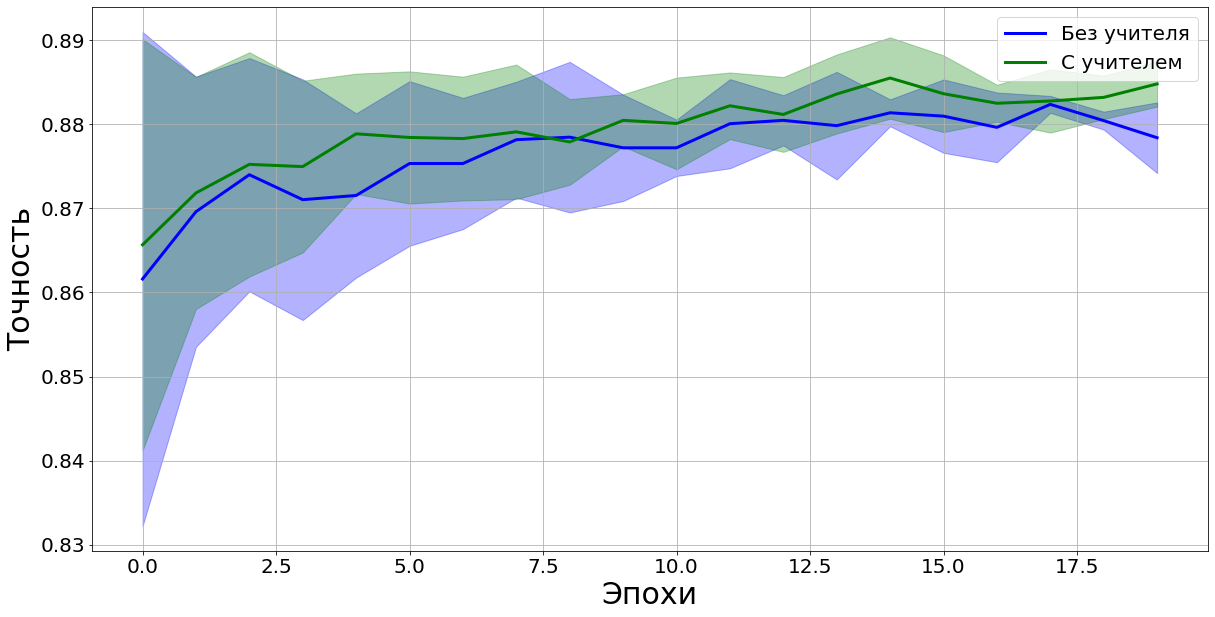
\includegraphics[width=0.5\textwidth]{results/acc}}
\subfloat[]
{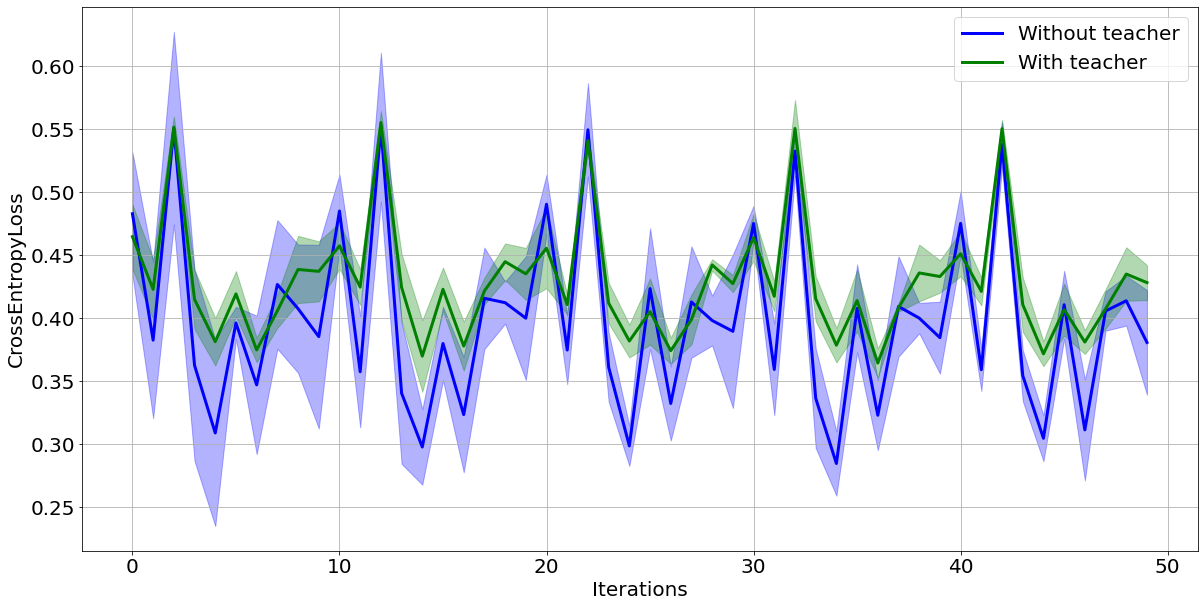
\includegraphics[width=0.5\textwidth]{results/loss}}\\
\caption{Качество аппроксимации на тестовой выборке. Все результаты усреднены по 5 запускам. a) accuracy; b) CrossEntropyLoss между истинными и предсказанными учеником метками}
\end{figure}\\
На рис.1а показан график зависимости метрики accuracy на тестовой выборке между истинными метками объектов и вероятностями, предсказанными моделью ученика.\\
На рис.1б показан график зависимости кросс-энтропии на тестовой выборке между истинными метками объектов и вероятностями, предсказанными моделью ученика.\\
На графиках видно, что модель, использующая метки учителя, показывает лучшее значение accuracy, при этом наблюдается значительное снижение кросс-энтропийной ошибки.


\paragraph{Обучение на малоресурсной части.}
Модель учителя обучается на многоресурсной части, а модель ученика обучается на малоресурсной части.\\
\begin{figure}[h!t]\center
\subfloat[]
{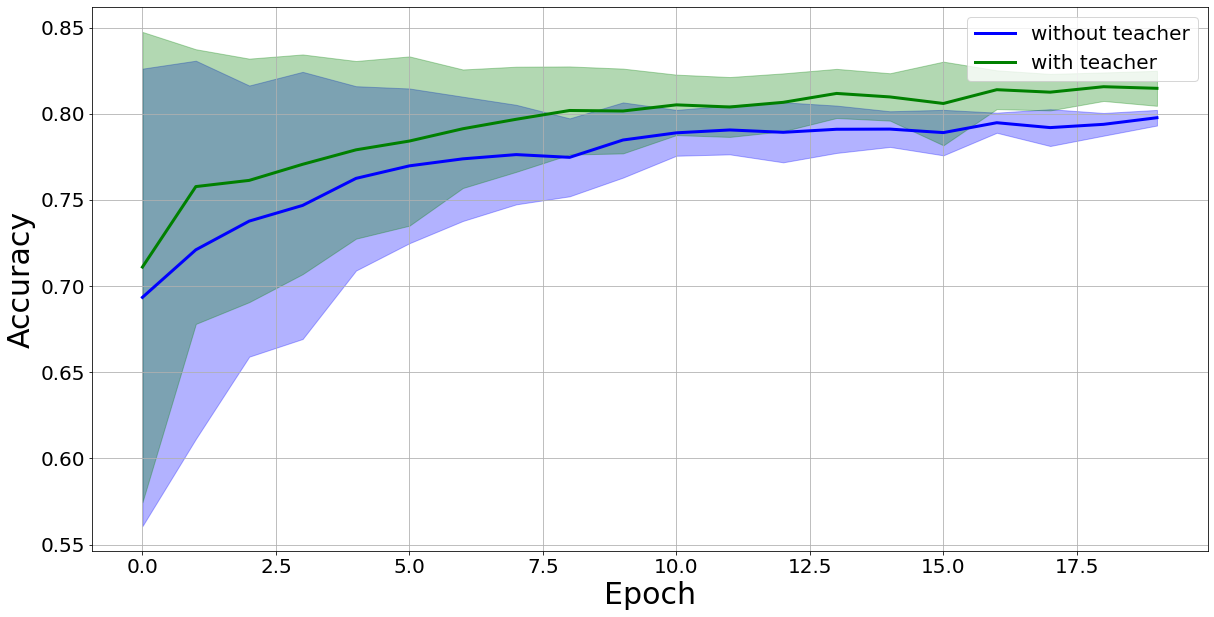
\includegraphics[width=0.5\textwidth]{results/small_acc}}
\subfloat[]
{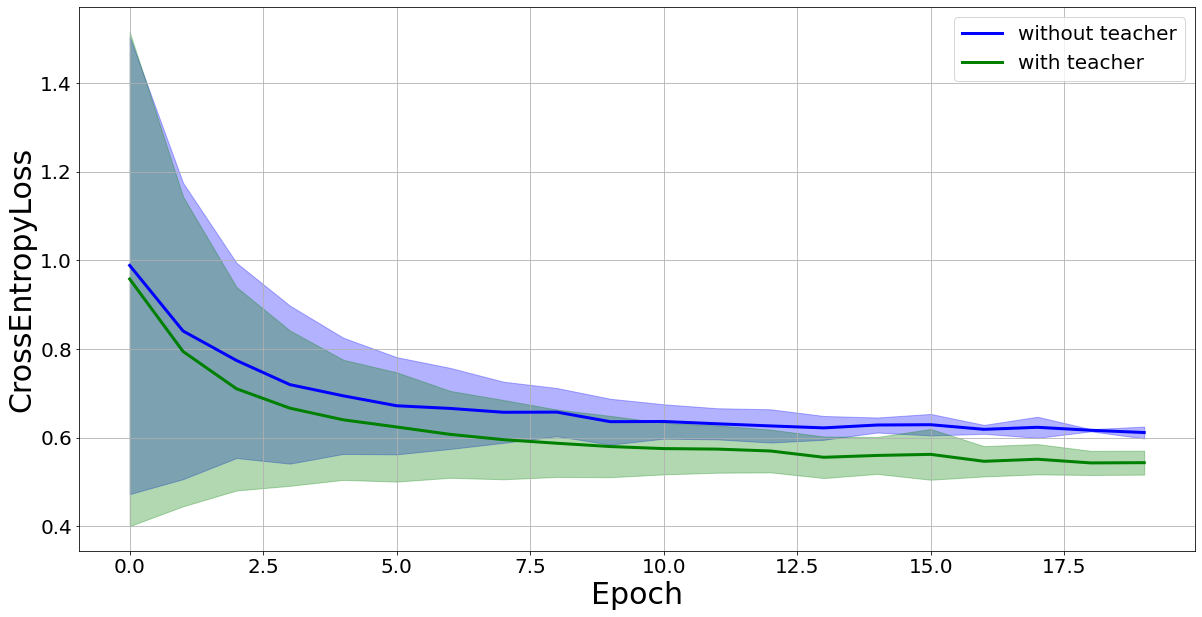
\includegraphics[width=0.5\textwidth]{results/small_loss}}\\
\caption{Качество аппроксимации на тестовой выборке. Все результаты усреднены по 5 запускам. a) accuracy; b) CrossEntropyLoss между истинными и предсказанными учеником метками}
\end{figure}\\
На рис.2а показан график зависимости метрики accuracy на тестовой выборке между истинными метками объектов и вероятностями, предсказанными моделью ученика.\\
На рис.2б показан график зависимости кросс-энтропии на тестовой выборке между истинными метками объектов и вероятностями, предсказанными моделью ученика.\\
На графиках видно, что модель, использующая метки учителя, показывает лучшее значение accuracy, при этом наблюдается снижение кросс-энтропийной ошибки.

\newpage
\paragraph{Обучение на выборке с шумом.}
Добавим к многоресурсной части нормальный шум $\mathcal{N}\bigr(0,\frac{1}{10}\bigr)$ и обучим на нем модель учителя. Модель ученика обучается на малоресурсной части без шума.
\begin{figure}[h!t]\center
{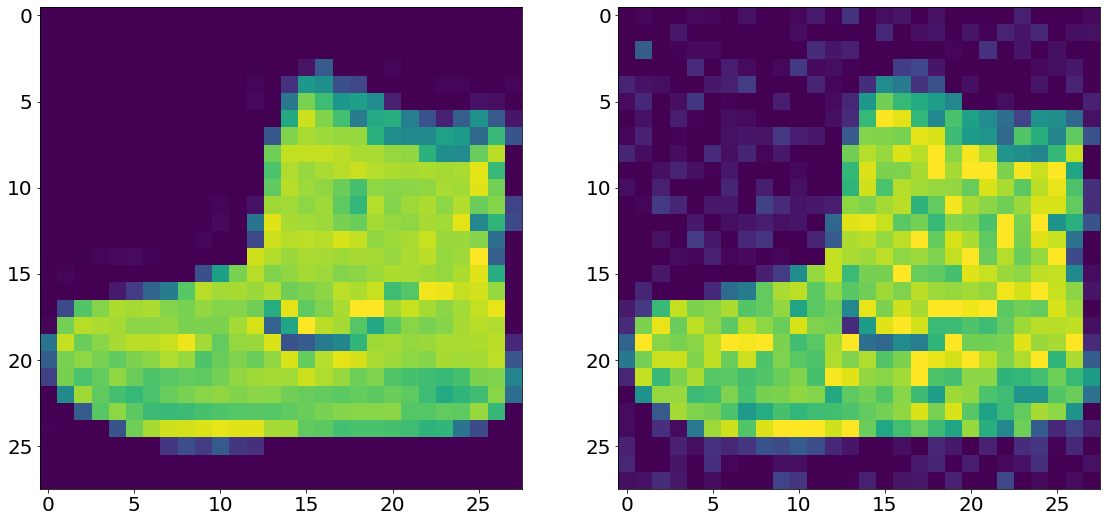
\includegraphics[width=0.5\textwidth]{results/noise}}
\caption{Сравнение объекта выборки до и после добавления шума}
\end{figure}\\

\begin{figure}[h!t]\center
\subfloat[]
{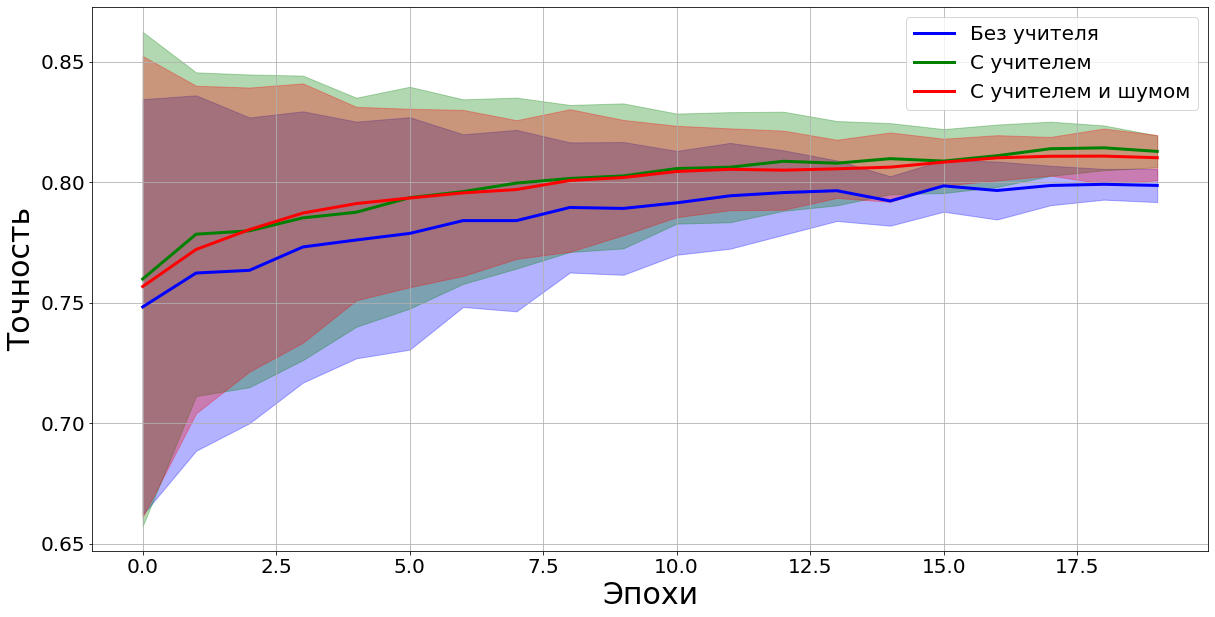
\includegraphics[width=0.5\textwidth]{results/noise_acc}}
\subfloat[]
{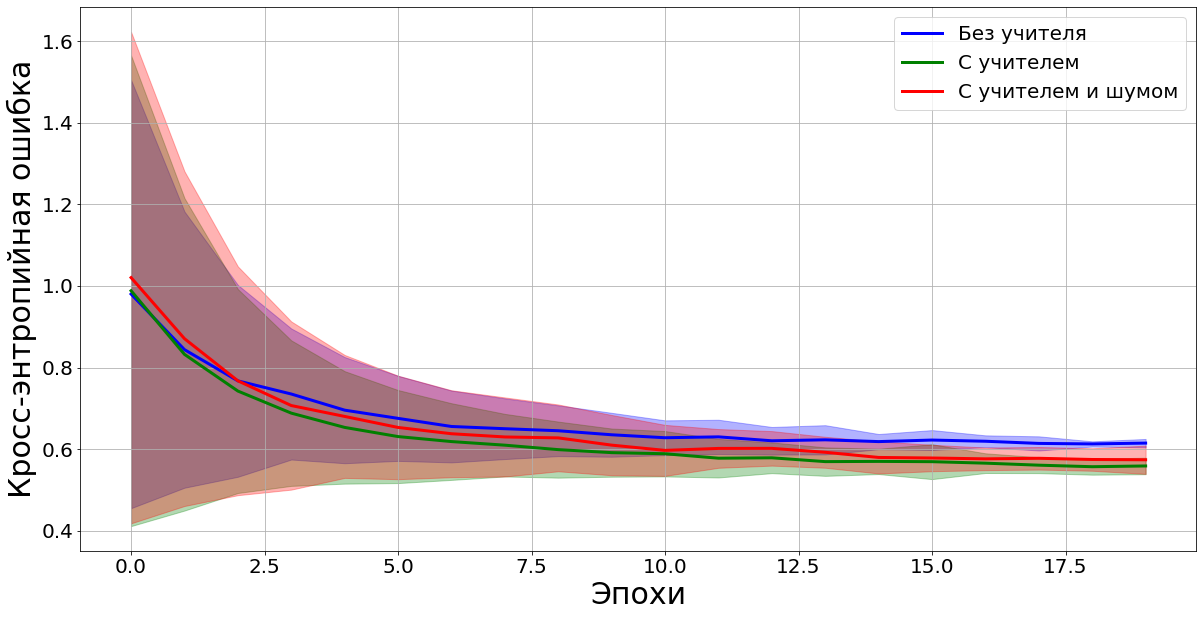
\includegraphics[width=0.5\textwidth]{results/noise_loss}}\\
\caption{Качество аппроксимации на тестовой выборке. Все результаты усреднены по 5 запускам. a) accuracy; b) CrossEntropyLoss между истинными и предсказанными учеником метками}
\end{figure}\\
На рис.4а показан график зависимости метрики accuracy на тестовой выборке между истинными метками объектов и вероятностями, предсказанными моделью ученика.\\
На рис.4б показан график зависимости кросс-энтропии на тестовой выборке между истинными метками объектов и вероятностями, предсказанными моделью ученика.\\
На графиках видно, что значения accuracy и CrossEntropyLoss модели, использующей метки учителя на выборке с шумом, лежат между соответствующими значениями для модели без учителя и для модели, использующей метки учителя на выборке без шума.\\
Получаем, что шум в выборке не влияет на качество.

\paragraph{Обучение на выборке с dilation.}
Применим к многоресурсной части сверточное преобразование с параметром $\text{dilation}=2$ и обучим на нем модель учителя. Модель ученика обучается на малоресурсной части.\\
\begin{figure}[h!t]\center
{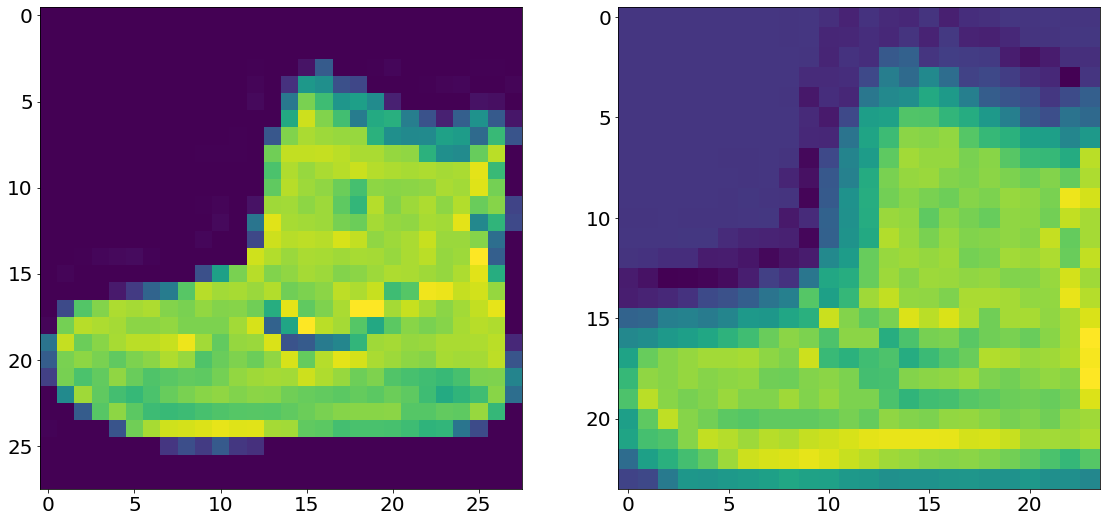
\includegraphics[width=0.5\textwidth]{results/dilation}}
\caption{Сравнение объекта выборки до и после преобразования}
\end{figure}\\

\begin{figure}[h!t]\center
\subfloat[]
{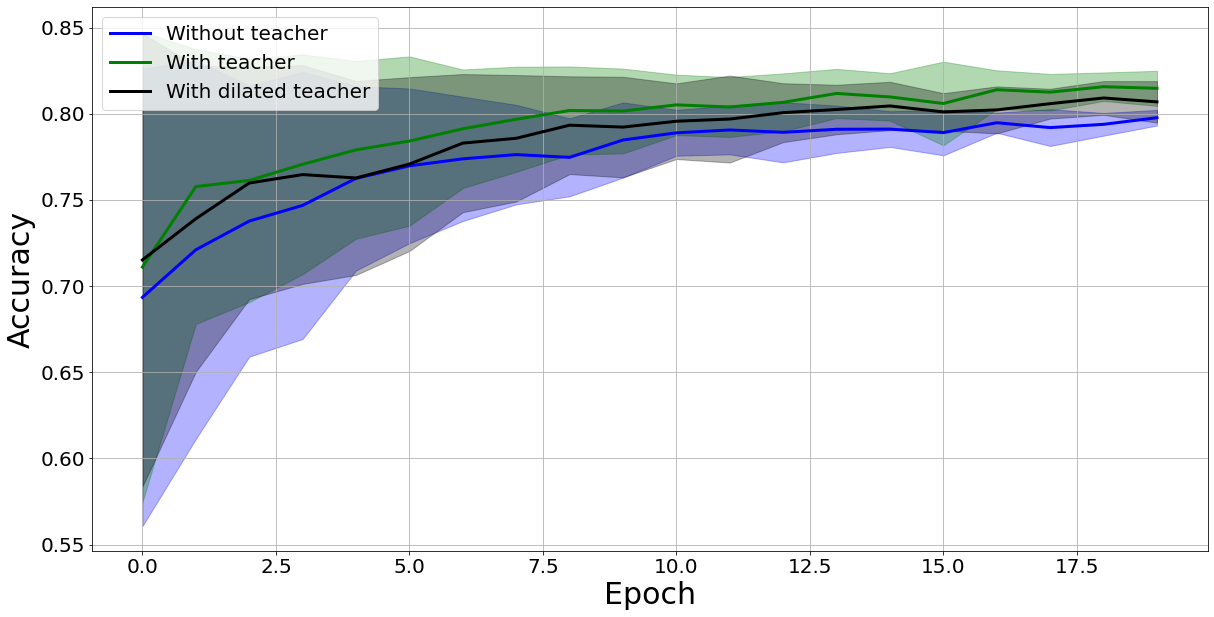
\includegraphics[width=0.5\textwidth]{results/dilation_acc}}
\subfloat[]
{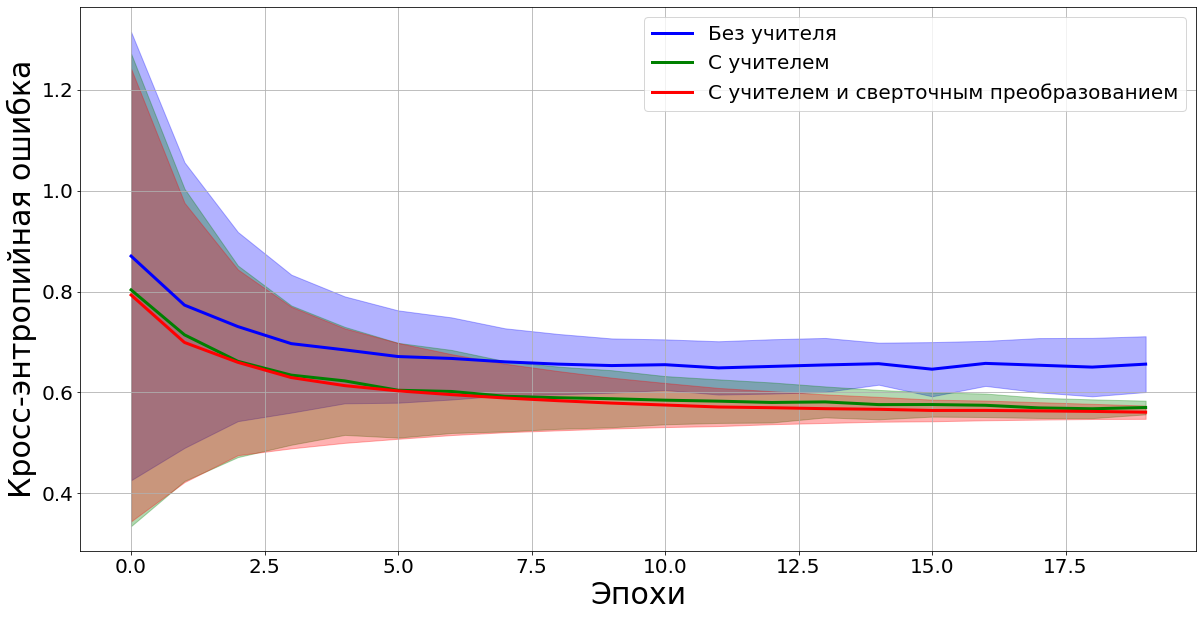
\includegraphics[width=0.5\textwidth]{results/dilation_loss}}\\
\caption{Качество аппроксимации на тестовой выборке. Все результаты усреднены по 5 запускам. a) accuracy; b) CrossEntropyLoss между истинными и предсказанными учеником метками}
\end{figure}\\
На рис.6а показан график зависимости метрики accuracy на тестовой выборке между истинными метками объектов и вероятностями, предсказанными моделью ученика.\\
На рис.6б показан график зависимости кросс-энтропии на тестовой выборке между истинными метками объектов и вероятностями, предсказанными моделью ученика.\\
На графиках видно, что значения accuracy и CrossEntropyLoss модели, использующей метки учителя на выборке с преобразованием, лежат между соответствующими значениями для модели без учителя и для модели, использующей метки учителя на выборке без преобразования.

\subsection{Вариационный автокодировщик}
В качестве преобразования элементов выборки FashionMNIST~\cite{FMNIST} в элементы выборки MNIST~\cite{MNIST} используем модель вариационного автокодировщика~\cite{VAE}, аппроксимирующую отображение $\varphi$.
\paragraph{Базовая модель автокодировщика.} Данная модель состоит из двух частей. Сначала строится вероятностоное распределение в скрытом пространстве, которое позволяет генерировать кодовые представления для одного объекта. Далее с помощью декодировщика строится вероятностное распределение, позволяющее генерировать реконструкци исходного объекта.\\
\\
$\mathbf{q_{\alpha}(z|x)}$-вероятностный кодировщик\\
$\mathbf{p_{\beta}(\hat{x}|z)}$-вероятностный декодировщик\\
$\mathbf{\mathcal{L}_{\text{VAE}}(\alpha, \beta)=\sum\limits_{i=1}^{l}\text{E}_{z\sim q_{\alpha}(z|x_{i})}\log{p_{\beta}(x_{i}|z)}dz-\text{KL}(q_{\alpha}(z|x_{i})||p(z))}$,\\
\\
$\mathbf{p(z)\sim \mathcal{N}(0,\sigma^{2}\mathbf{I})}$ - априорное распределение\\
\\
Получаем оптимизационную задачу:
$$\hat{\alpha}, \hat{\beta} = \arg\max_{\alpha, \beta} \mathcal{L}(\alpha, \beta).$$

\newpage
\paragraph{Генерация отображения из FashionMNIST в MNIST.}
Воспользуемся моделью вариационного автокодировщика~\cite{VAE} для преобразования изображений одежды из выборки FashionMNIST~\cite{FMNIST} в изображения цифр на основе выборки MNIST~\cite{VAE}.\\
Создадим синтетическую выборку, где каждому изображению одежды будет соответстовать случайное изображение цифры из того же класса.\\
\begin{figure}[h!t]\center
\subfloat[]
{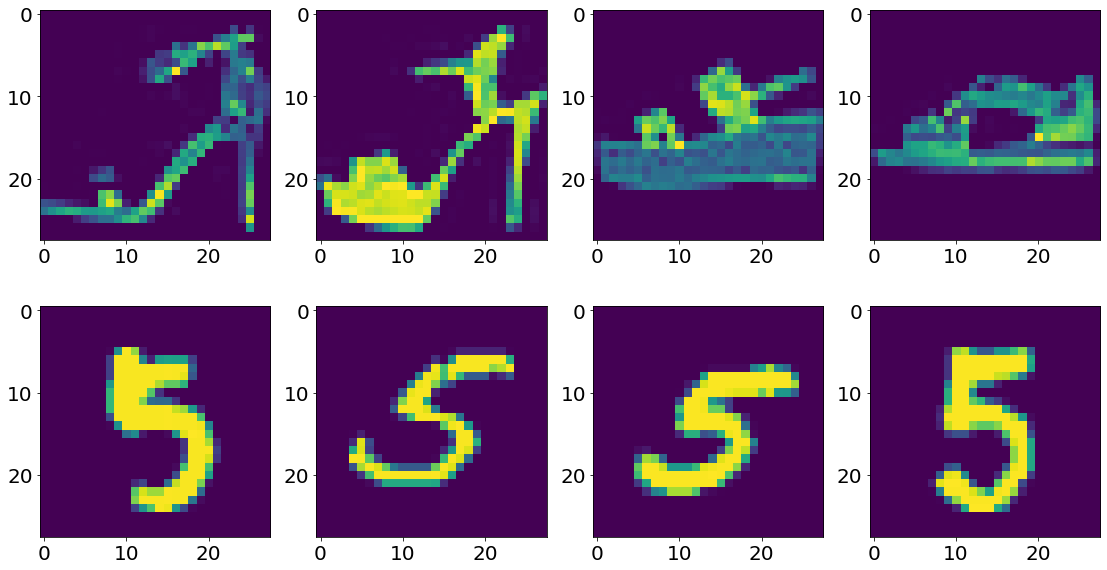
\includegraphics[width=0.4\textwidth]{results/fmnist_random_mnist.png}}
\qquad
\subfloat[]
{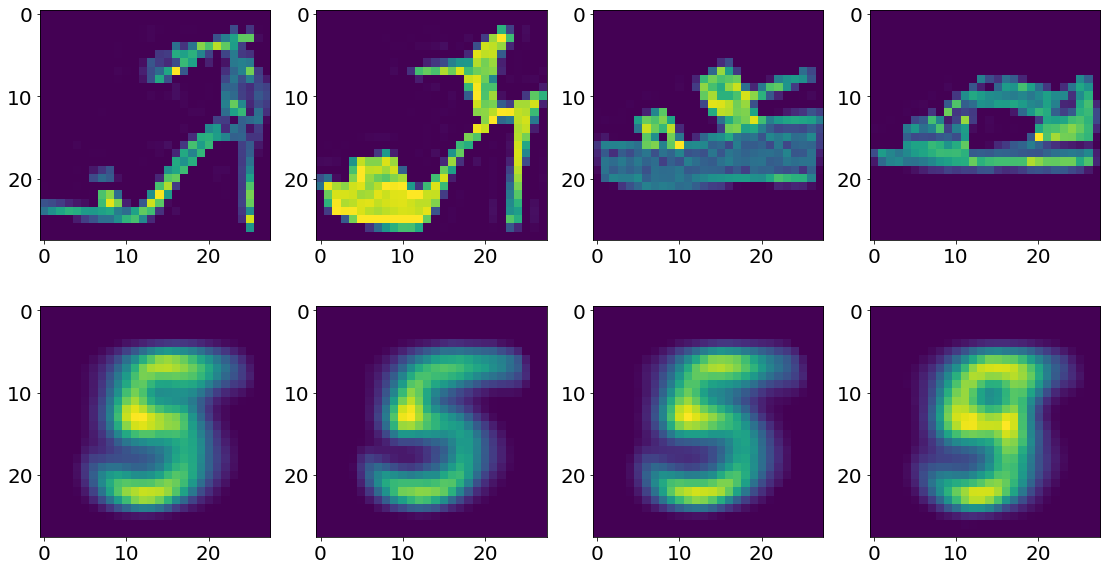
\includegraphics[width=0.4\textwidth]{results/fmnist_vae_mnist.png}}\\
\caption{a) Объекты синтетический выборки; b) Объекты исходной выборки до и после работы автокодировщика}
\end{figure}\\
Далее воспользуемся моделью вариационного автокодировщика~\cite{VAE}, состоящего из одного кодировщика и двух декодировщиков, соответствующих генерации объектов цифр или одежды. Используем модель с размером скрытого представления, равным 64.\\
На основе данной выборки обучим модель вариационного автокодировщика~\cite{VAE}, минимизируя ошибку между выходом модели и исходным значением --- изображением одежды и ошибку между выходом модели и целевым значением --- изображением цифр, соответствующего исходному объекту.\\
Получили модель, способную генеририровать семейство новых объектов - изображений цифры или изображений одежды для одного и того же изображения одежды.
\newpage
Посмотрим также на изменение выхода модели при изменении случайного вектора в скрытом представлении. Для визуализации построим скрытое представление размерности 2:\\

\begin{figure}[h!t]\center
\subfloat[]
{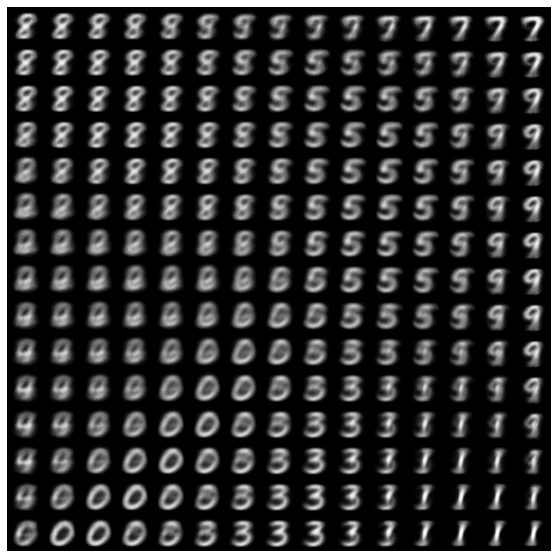
\includegraphics[width=0.4\textwidth]{results/decoder_digits.png}}
\qquad
\subfloat[]
{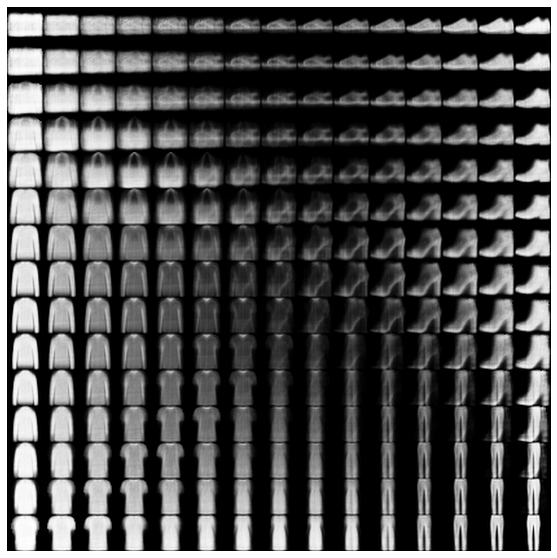
\includegraphics[width=0.4\textwidth]{results/decoder_fashion.png}}\\
\caption{Зависимость выхода модели от изменения вектора в скрытом представлении для генерации a) цифр; b) одежды}
\end{figure}\\

\subsection{Анализ качества модели, предложенной на основе вариационного автокодировщика}
Будем обучать модель учителя на выборке MNIST~\cite{MNIST}, а модель ученика на выборке FashionMNIST~\cite{FMNIST}. При этом при обучении модели ученика будем использовать метки учителя, подавая ему на вход выход вариационного автокодировщика~\cite{VAE}, переводящего изображения одежды в изображения цифр.\\
Также для сравнения покажем качество аппроксимации без использования вариационного автокодировщика~\cite{VAE}: модель ученика обучается на выборке FashionMNIST~\cite{FMNIST}, модель учителя обучается на выборке MNIST~\cite{MNIST} и используется при обучении ученика, получая на вход изображения одежды без преобразования вариационным автокодировщиом.\\

\begin{figure}[h!t]\center
\subfloat[]
{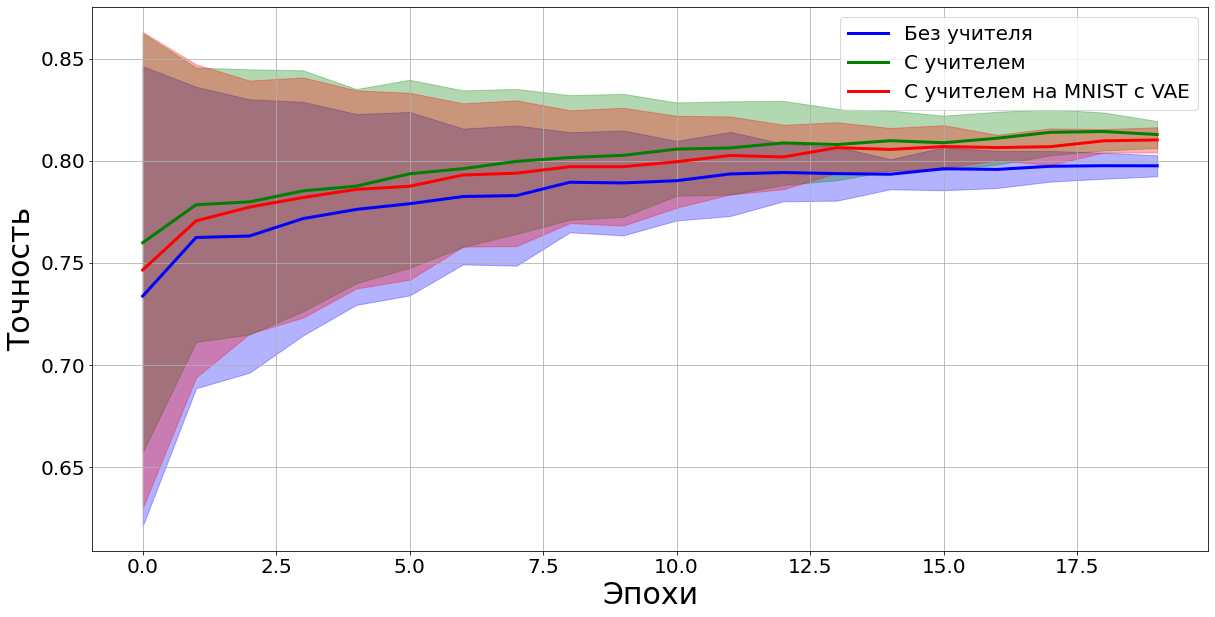
\includegraphics[width=0.5\textwidth]{results/vae_acc}}
\subfloat[]
{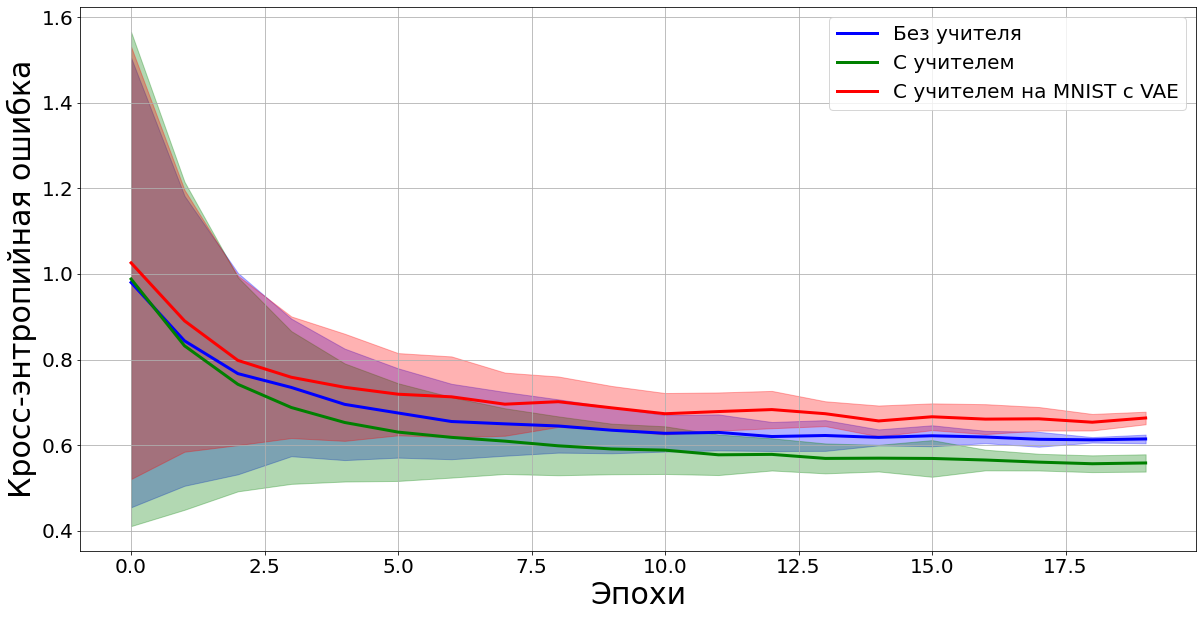
\includegraphics[width=0.5\textwidth]{results/vae_loss}}\\
\caption{Качество аппроксимации при использовании VAE на малодоменной выборке. Все результаты усреднены по 5 запускам. a) accuracy; b) CrossEntropyLoss между истинными и предсказанными учеником метками}
\end{figure}\\

\begin{figure}[h!t]\center
\subfloat[]
{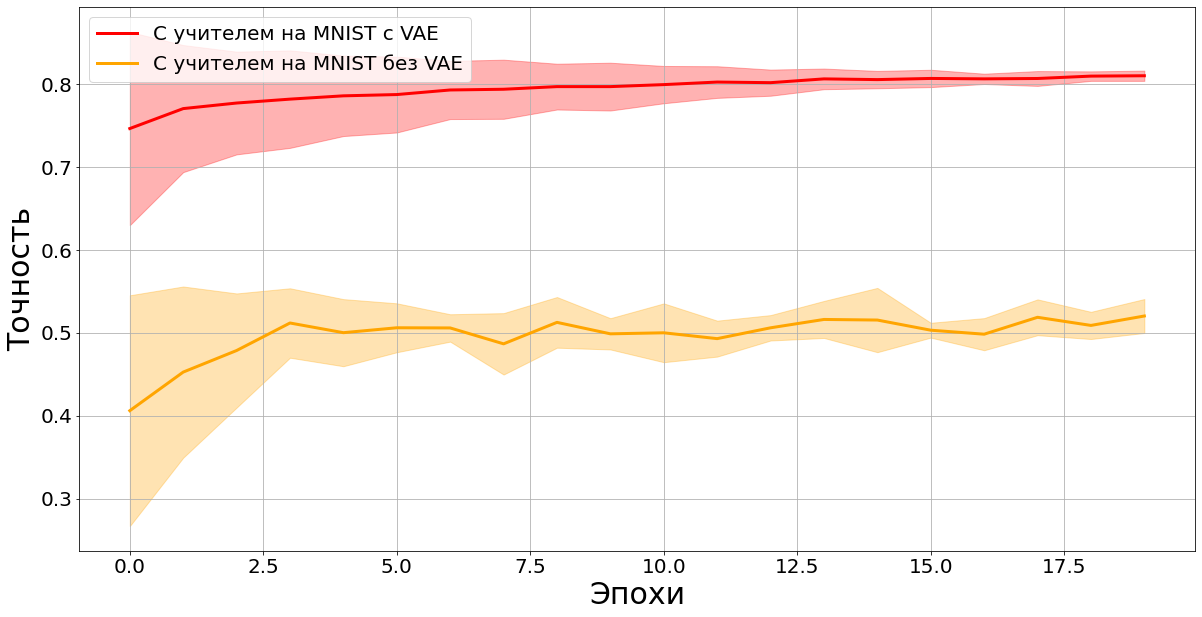
\includegraphics[width=0.5\textwidth]{results/vae_acc_comparison}}
\subfloat[]
{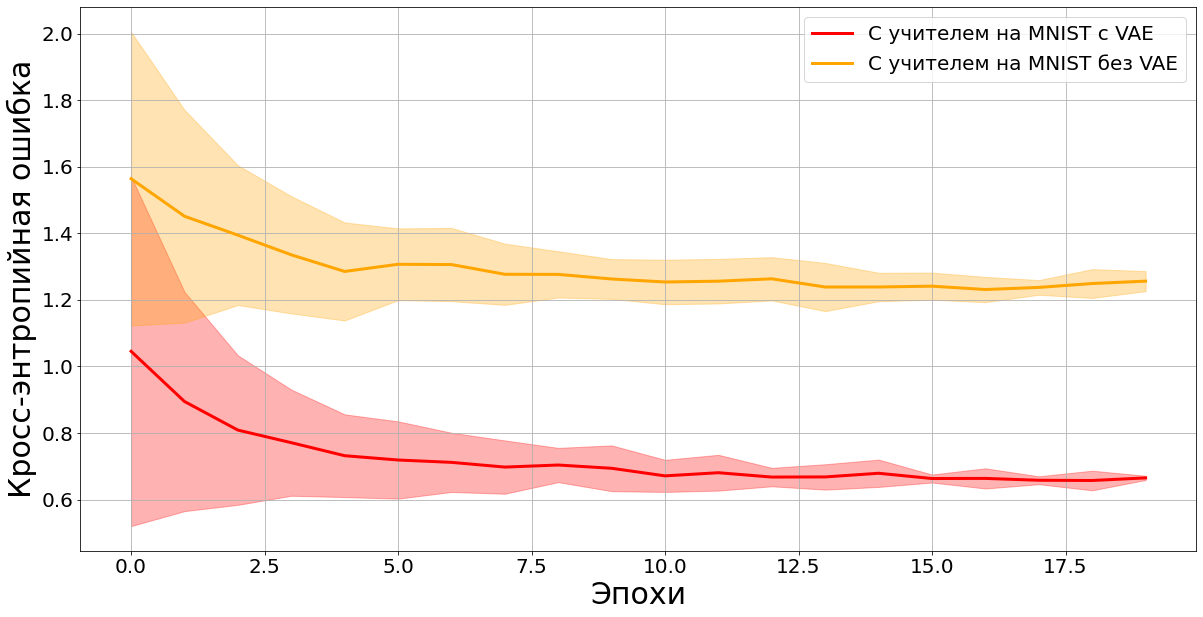
\includegraphics[width=0.5\textwidth]{results/vae_loss_comparison}}\\
\caption{Сравнение качества аппроксимации в зависимости от использования VAE на малодоменной выборке. Все результаты усреднены по 5 запускам. a) accuracy; b) CrossEntropyLoss между истинными и предсказанными учеником метками}
\end{figure}

На графиках видно, что без использования отображения $\varphi$ модель становится более шумной с явным понижением качества аппроксимации.

\newpage
\subsection{Анализ качества модели на расширенной синтетически сгенерированной выборке}
На основе малоресурсной части выборки сгенерируем новую выборку, сгенерировав для каждого объекта одежды 70 изображений цифр с помощью модели вариационного автокодировщика~\cite{VAE}. Далее разделим полученную выборку на две части: часть для обучения содержит 60000 объектов, тестовая часть содержит 10000 объектов.\\
Модель ученика обучается на малоресурсной части выборки FashionMNIST~\cite{FMNIST}, модель учителя на части для обучения сгенерированной расширенной выборки и используется при обучении ученика.

\begin{figure}[h!t]\center
\subfloat[]
{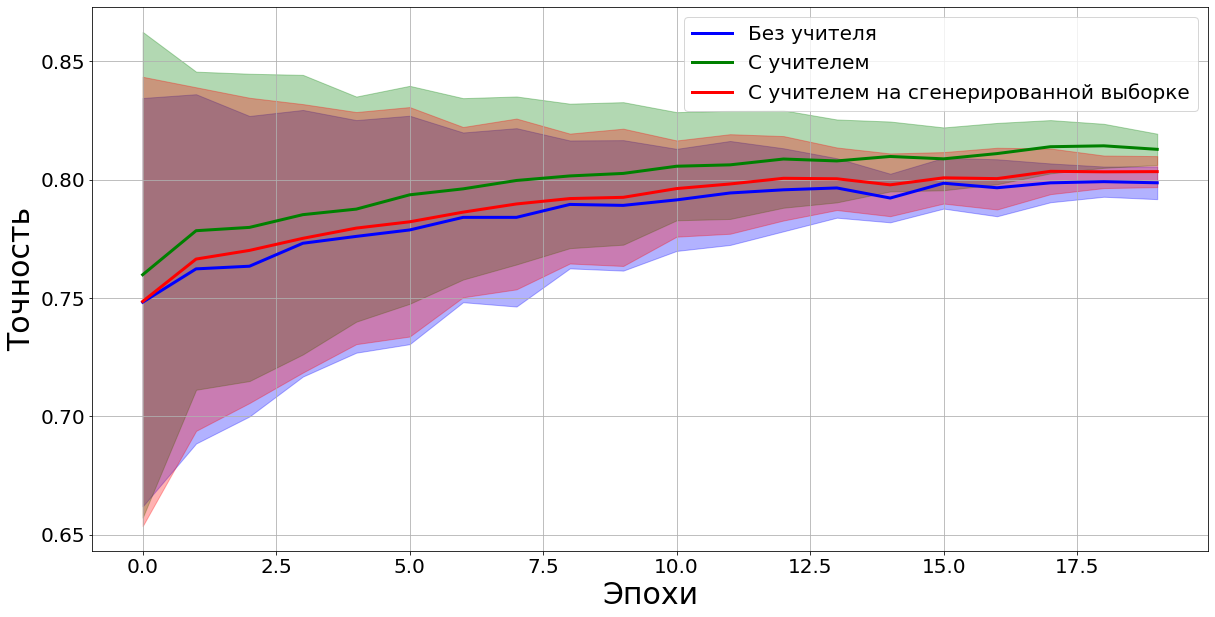
\includegraphics[width=0.5\textwidth]{results/ext_mnist_acc.png}}
\subfloat[]
{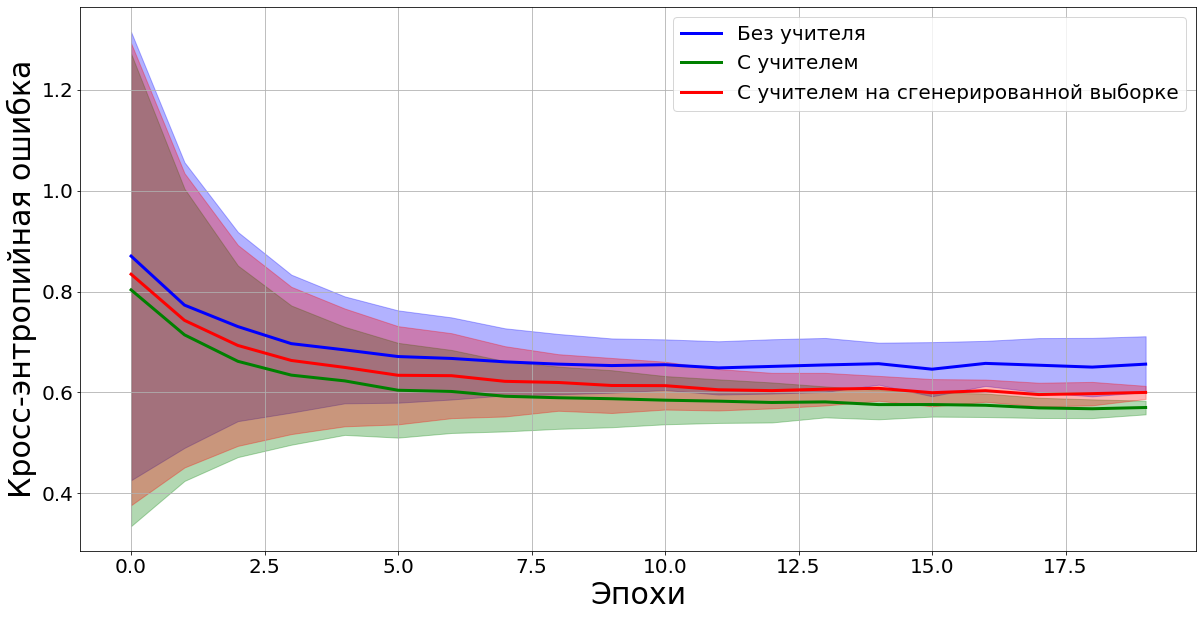
\includegraphics[width=0.5\textwidth]{results/ext_mnist_loss.png}}\\
\caption{Качество аппроксимации на тестовой выборке. Все результаты усреднены по 5 запускам. a) accuracy; b) CrossEntropyLoss между истинными и предсказанными учеником метками}
\end{figure}\\

На графиках видно, что значения accuracy и CrossEntropyLoss модели, использующей метки учителя, обученного на сгенерированной расширенной выборке, лежат между соответствующими значениями для модели без учителя и для модели, использующей метки учителя, обученного на многоресурсной части выборки.